\documentclass[11pt, a4paper]{article}
\usepackage[utf8]{inputenc}
\usepackage[T1]{fontenc}
\usepackage[charter]{mathdesign} % Elegant, readable font
\usepackage{geometry}
\geometry{margin=1in}
\usepackage{enumitem}
\usepackage{amsmath}
\usepackage{booktabs}
\usepackage{hyperref}
\usepackage{graphicx} % Required for inserting images (put this in your preamble)
\usepackage{subfig}
\usepackage{comment}
\usepackage{tikz}
\usepackage{xcolor}
\usepackage{colortbl}

\makeatletter
\renewcommand{\maketitle}{
  \begin{flushleft}
    {\huge \textbf{\@title} \par}
    \vspace{0.5cm}
    {\large \@author \par}
    \vspace{0.2cm}
    {\@date \par}
    \vspace{0.2cm}
    \hrule
  \end{flushleft}
}
\makeatother

% FIXED: Removed the stray \\[-0.2em]} from this line
\title{\LARGE\textbf{Assignment 5: Lenia -- An artificial life}} 
\author{
    Plabon Shaha and Guillem Masdemont \\ 
    \small University of Ljubljana, Spring Semester, EMAI Cohort 25--27 
}

\begin{document}

\maketitle

\begin{enumerate}
    \item[\textbf{Evaluation}] We use different versions to evaluate performance metrics.

\definecolor{v1color}{HTML}{1F77B4}
\definecolor{v2color}{HTML}{FF7F0E}
\definecolor{v3color}{HTML}{2CA02C}
\definecolor{v4color}{HTML}{D62728}
\definecolor{v5color}{HTML}{9467BD}
\definecolor{v6color}{HTML}{8C564B}

\newcommand{\versionbox}[2]{%
    \begin{tikzpicture}
        \node[
            draw=#1, line width=1.4pt,
            rounded corners=5pt,
            fill=#1!10,
            minimum width=3.9cm,
            minimum height = 2.0cm,
            text width=3.6cm,
            align=center,
            inner sep=7pt
        ] {
            \textcolor{#1}{\textbf{\footnotesize #2}}
        };
    \end{tikzpicture}%
}

\begin{table}[h]
\centering
\setlength{\tabcolsep}{5pt}
\renewcommand{\arraystretch}{1.3}
\begin{tabular}{ccc}
    \versionbox{v1color}{Row distribution (1 process, 1-2 nodes)} &
    \versionbox{v2color}{Row distribution (16 processes, 1-2 nodes)} &
    \versionbox{v3color}{Block distribution (16 processes, 1-2 nodes)} \\[8pt]

    \versionbox{v4color}{Block distribution + derived DT (16 processes, 1-2 nodes)} &
    \versionbox{v5color}{GPU (1 node, 1-2 GPU)} &
\end{tabular}
\caption{Overview of Lenia Simulation Parallel Configurations} % Added caption for good practice with labels
\label{tab:version_grid}
\end{table}

\begin{figure}[h]
    \centering
    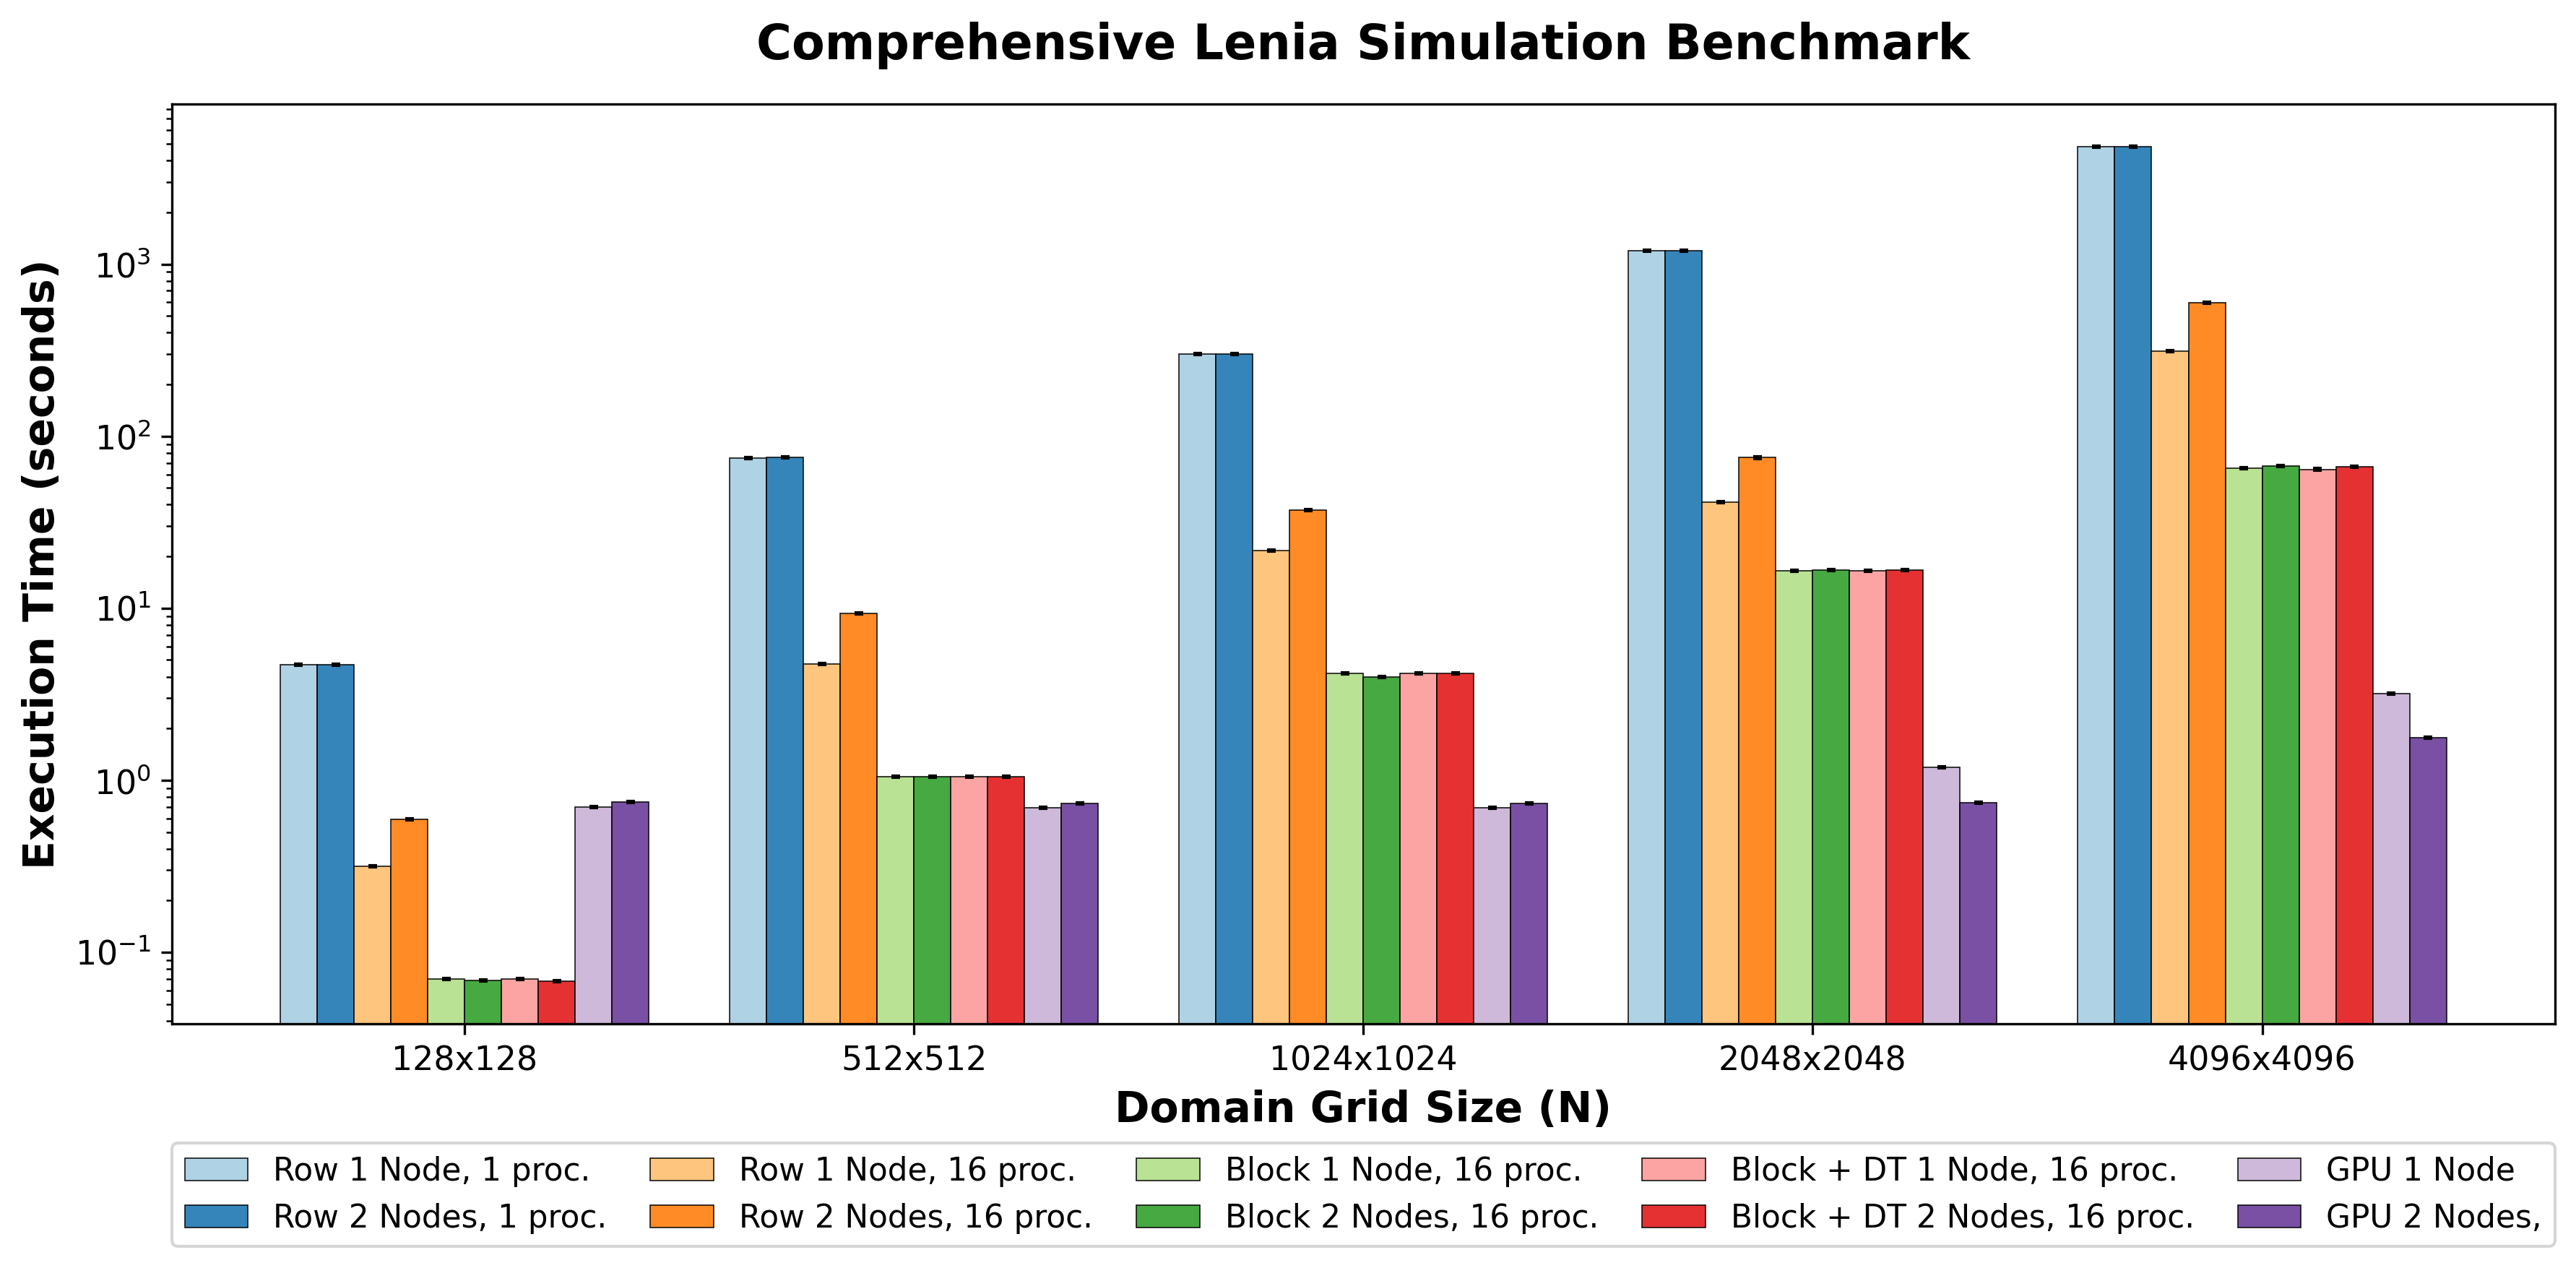
\includegraphics[width=1.05\textwidth]{lenia_interleaved_legend.png}
    \caption{Performance comparison of the aforementioned optimization layers.}
    \label{fig:performance_plots}
\end{figure}

For Row distribution, splitting across 2 nodes slows down performance because full-width halo rows must travel over a slower network instead of fast intra-node shared memory. Block distribution outperforms row distribution because its 4×4 grid layout sends half as much communication data per process. Using MPI Derived Types (Block+DT) yields a negligible difference over manual packing because the creation overhead completely offsets any packing efficiency. Block distribution significantly reduces halo data, scaling to 2 nodes remains cheap enough to keep performance nearly identical to a single node. Finally, GPUs are heavily bottlenecked by launch and transfer overheads on small grids ($N=128$), but their massive parallelism completely dominates large scales ($N=4096$). A second GPU succeeds only after there is enough compute work to offset the split costs.




\item Now, we increase the width of the border area exchanged between processes so by performing additional computations, we can exchange data only every second, third, etc. iteration. We show the results for the 2048 pixel image and 4,16, 34 processes. The results are presented in the following image

\begin{figure}[h]
    \centering
    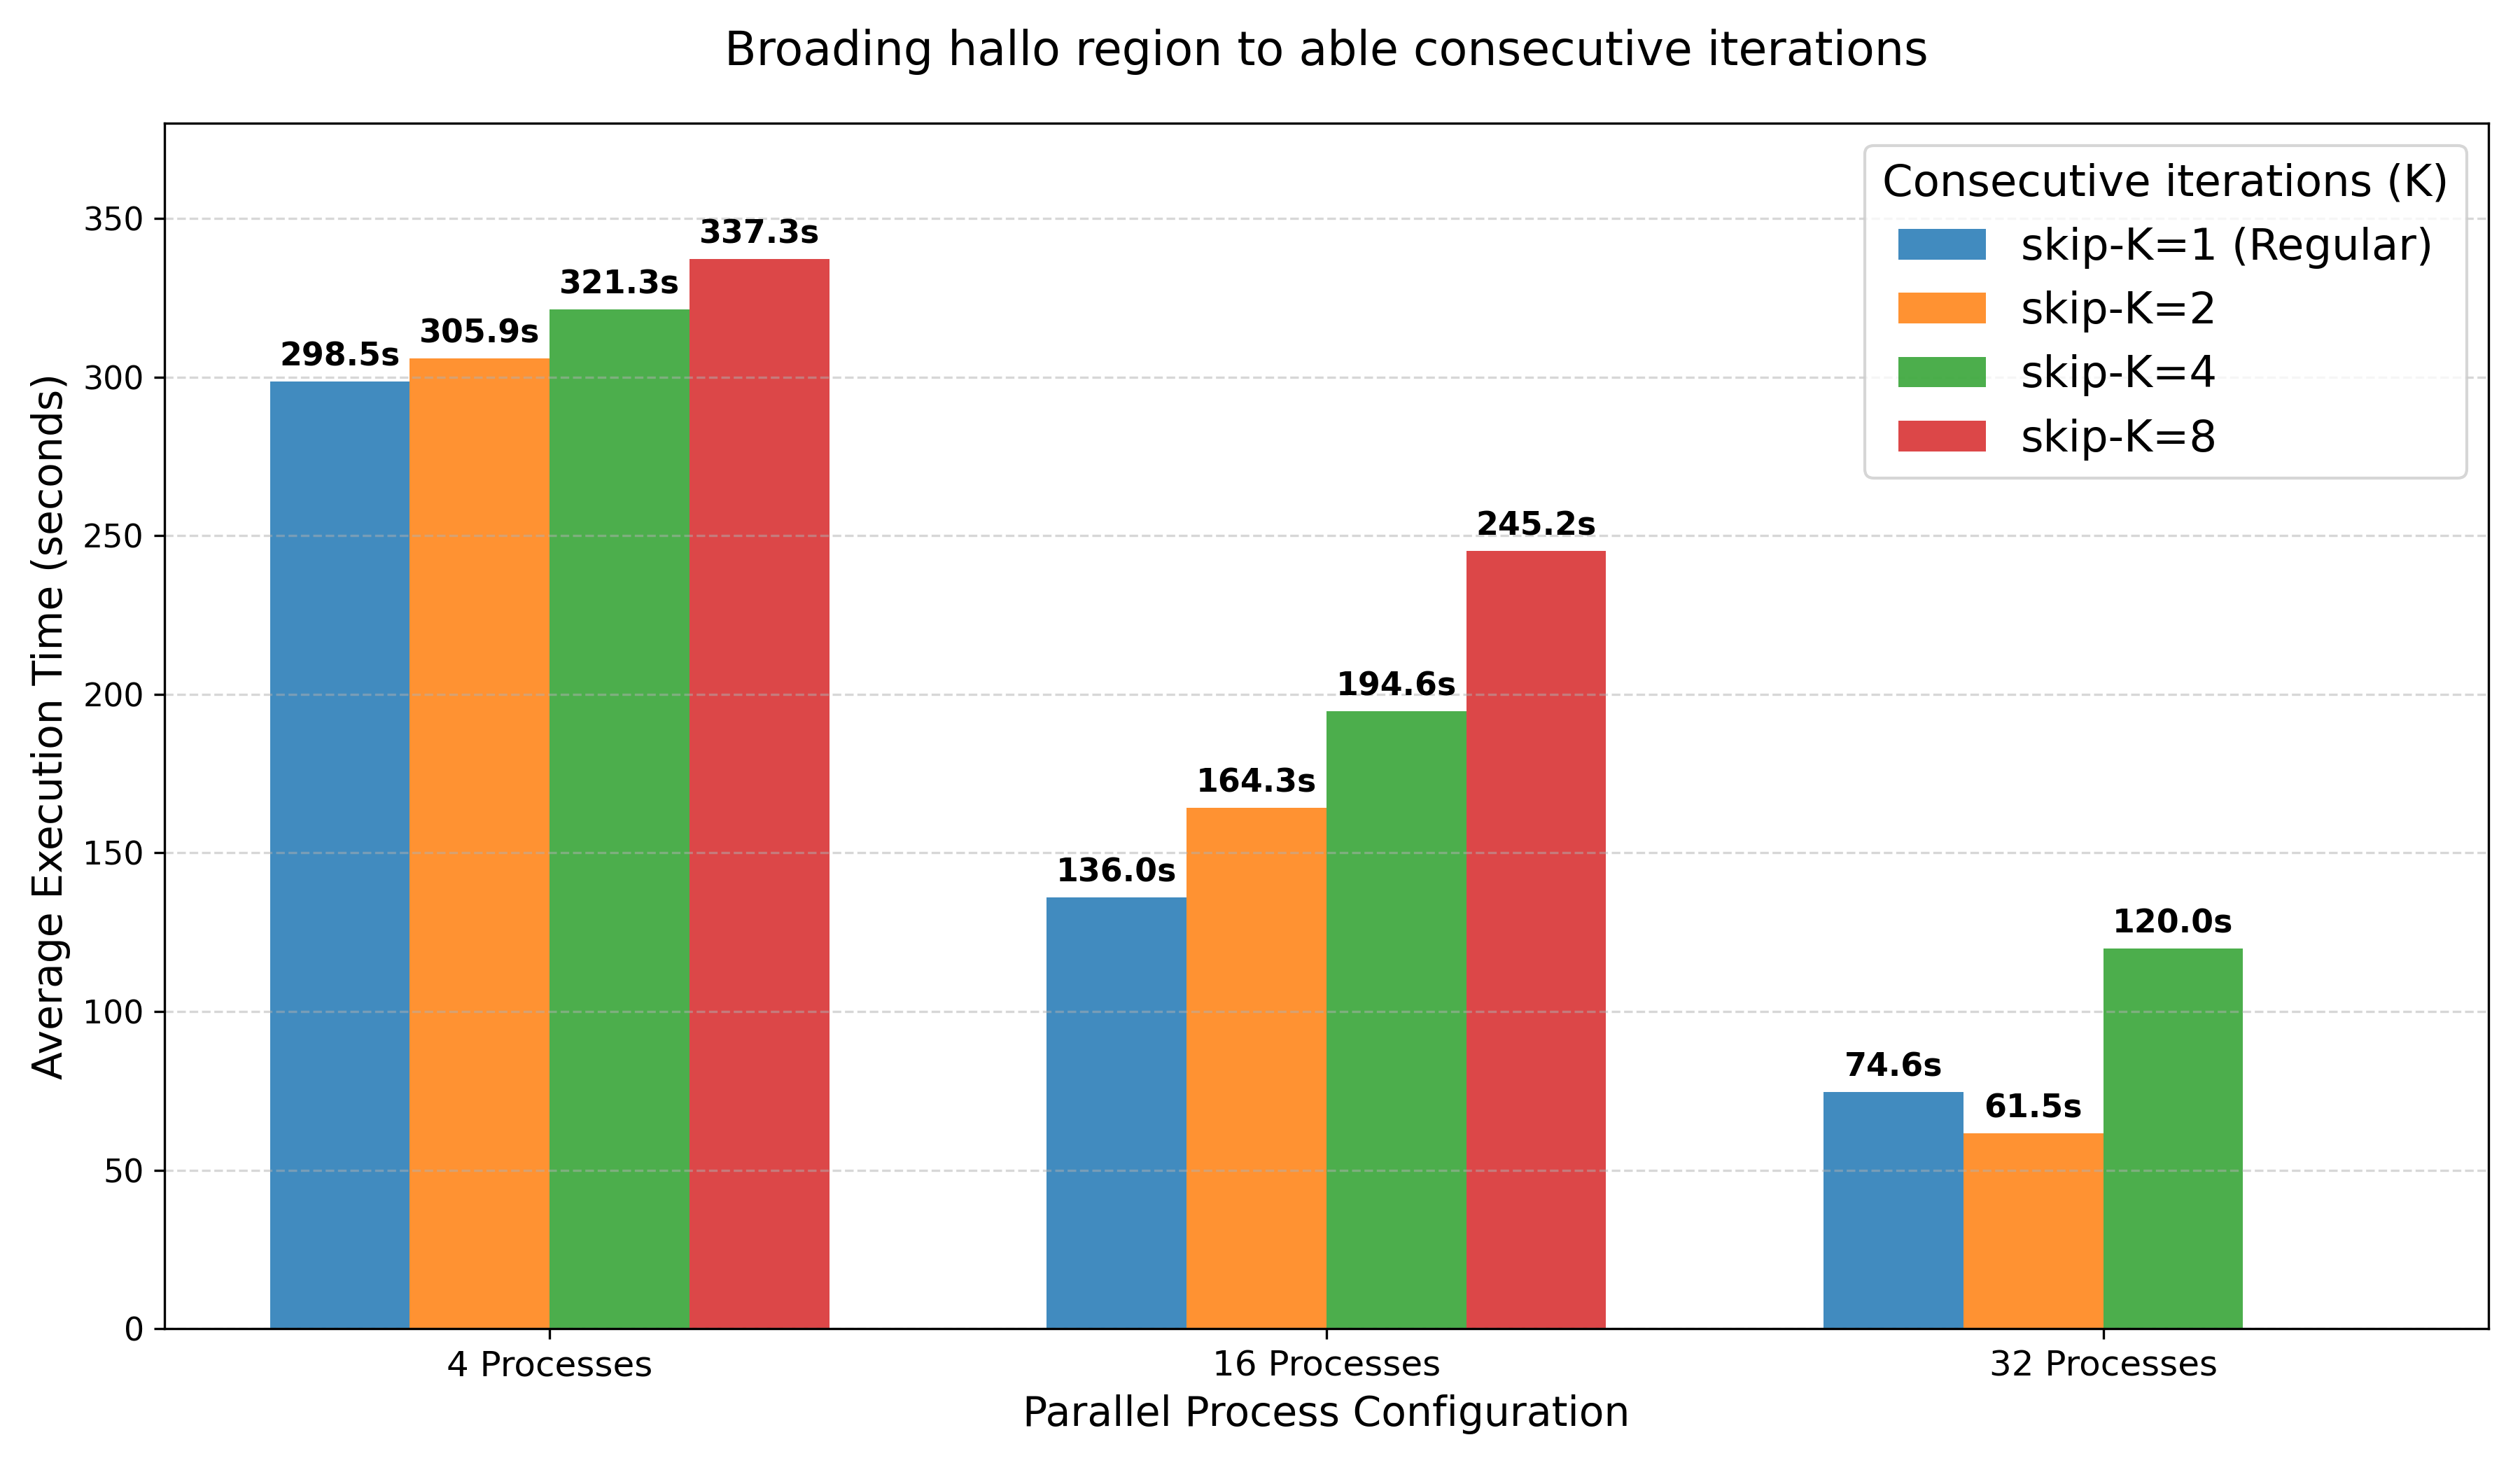
\includegraphics[width=1.05\textwidth]{lenia_skip_k_benchmark.png}
    \caption{Performance comparison of the aforementioned optimization layers.}
    \label{fig:skip_k}
\end{figure}

Widening the halo region by a factor of $K$ trades a larger local computation burden for fewer but larger MPI exchanges. For the $K=1$ baseline, communication is already cheap at high process counts (32 processes), leaving very little network overhead to amortize. Consequently, using higher $K$ factors always hurts performance at 4 and 16 processes because calculating a wider border forces processes to perform massive redundant computations that their neighbors would have completed anyway. Since each process already owns a large chunk of the domain at lower process counts, this extra work quickly outweighs any communication savings. The only exception occurs at 32 processes with $K=2$, where the local domain strips are so thin that communication overhead is high enough that skipping every other exchange actually saves time. However, setting $K=4$ or $K=8$ overcorrects even at this scale, causing redundant edge computations to dominate and drive runtimes back up.

\end{enumerate}

\end{document}